\documentclass[pdftex,12pt,a4paper]{article}
\usepackage[pdftex]{graphicx}
\usepackage{xcolor}
\usepackage{marginnote}
\usepackage{enumitem}
\usepackage[bottom=1.5cm, outer=5cm, inner=2cm, heightrounded,
marginparwidth=4cm, marginparsep=0.5cm]{geometry}

\begin{document}
    % Custom title page
    \begin{titlepage}
        \begin{center}
            
\includegraphics[width=5cm]{figures/kulogo}\\[1cm]
            {\Large \bfseries
                Spring 2014\\
                Computer Networks\\
                CMPE323\\[1cm]
            }
            {\large \bfseries
                \noindent Laboratory Experiment No. 8: Introduction to Firewalls\\[1cm]
            }
        \end{center}

        \noindent \textbf{Aims and Objectives:}
            \begin{itemize}[leftmargin=4cm]
                \item Introducing stateless network firewalls,
                \item and stateful firewalls.
            \end{itemize}
            \vspace{0.5cm}

        \noindent \textbf{Materials Required:}
            \begin{itemize}[leftmargin=4cm]
                \item Network firewalls,
                \item PCs with Ethernet adapters,
                \item and straight-through/crossover/rollover cables.
            \end{itemize}
            \vspace{0.5cm}

        \noindent \textbf{Change Log:}
            \begin{itemize}[leftmargin=4cm]
                \item 22-4-2014: original document -- mkhonji.
                \item 23-4-2014: typo fixes  -- mkhonji.
            \end{itemize}
    \end{titlepage}
    \newpage

    % Lab script content
    \section{Introduction}
        Essentially, network firewalls are devices that reside in the pathways
        of communication networks and serve as filtering devices that decide
        which packets are allowed to pass.

        Figure \ref{fig:fw} shows an example of a case where a firewall is used
        to filter packets in order to achieve the following scenario:
        \begin{itemize}
            \item An internal network that has strict/regulated access
                to the Internet. Nodes in the internal network are usually
                regulated by network firewalls such that the nodes can only
                access Internet resources if the nodes have initiated the
                connection. In other words, nodes from the Internet cannot
                send packets to nodes in the internal network unless the
                packets were responses to requests that were originated by the
                nodes in the internal network.
            \item A demilitarized zone (DMZ) that is directly accessible
                from the Internet. Unlike nodes in the internal network, nodes
                in the DMZ can be accessed directly by nodes in the Internet
                without having DMZ nodes initiate the request first.
            \item And an external network which is in this case the Internet.
        \end{itemize}

        \begin{figure}[tbh]
            \centering
            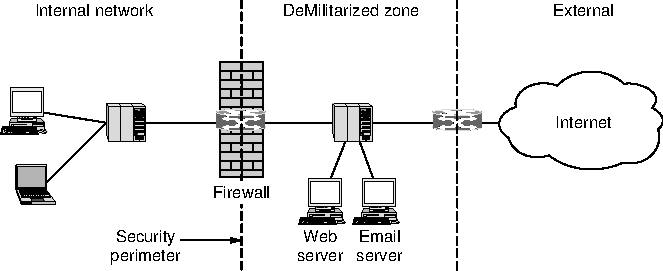
\includegraphics[width=0.9\textwidth]{figures/firewall}
            \caption{A firewall use case --- Source: Computer Networks 5$^{th}$
            Edition, 2010, by Andrew S. Tanenbaum and David J. Wetherall, page
            818.}
            \label{fig:fw}
        \end{figure}

        The following types of firewalls are common:
        \begin{itemize}
            \item Stateless firewalls --- such firewalls are among the oldest
                and simplest firewall types. They simply analyze packets and if
                certain patterns are matched, they decide whether to drop or
                permit them. The patterns that such firewalls analyze are often
                limited to layer 3 and layer 4 protocol headers (e.g. IP, TCP
                or UDP headers).
            \item Stateful firewalls --- similar to the stateful firewalls,
                except that they maintain a states table. Such states table
                allows the firewall to identify whether a packet is an initial
                packet or a response to a previous request.
            \item Application-layer firewalls --- similar to the previous types
                of firewalls, with the exception of being able to not only
                analyze layer 3 or layer 4 data, but the application layer data
                as well. For example, by analyzing the application-layer data,
                it can identify the application (e.g. FTP) even if it uses the
                port number of another application (e.g. TCP 80, which is for
                HTTP).
        \end{itemize}

        In this lab, we will only configure stateless and stateful firewalls
        using Cisco routers due to their availability in our lab. This is
        possible as our Cisco routers are not only routers, but also provide
        packet filtering capabilities (which is the functionality of a
        firewall).

    \section{Lab Preparation}
        \begin{enumerate}
            \item Erase the configuration of
                \texttt{R1}\footnote{\texttt{enable}, \texttt{erase
                startup-config}, \texttt{reload}, and make sure to answer
                \texttt{no} to all yes/no questions while hitting \emph{enter} for
                all \texttt{confirm} prompts.} and reboot \texttt{PC1} and
                \texttt{PC2}.
            \item Physically connect and configure IP addresses of the
                router\footnote{\texttt{enable}, \texttt{configure terminal},
                \texttt{interface Gi0/0}, \texttt{ip address <ip\_address>
                <subnet\_mask>}, \texttt{no shutdown}.} and the
                PCs\footnote{\texttt{ifconfig eth0
                <ip\_address>/<netmask\_bits>}} as depicted in Figure
                \ref{fig:labtop}.

                \begin{figure}[tbh]
                    \centering
                    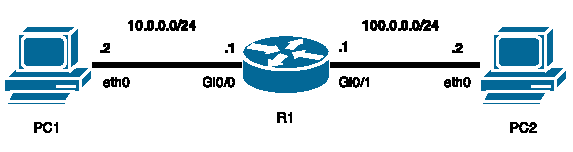
\includegraphics[width=0.9\textwidth]{figures/npat}
                    \caption{Lab topology.}
                    \label{fig:labtop}
                \end{figure}

           \item Add default routes\footnote{\texttt{route add -net
               0.0.0.0/0 gw <nexthop\_ip>}} to \texttt{PC1} and \texttt{PC2}.

           \item Run Wireshark on all the PCs.

           \item Using the \texttt{ncat}\footnote{\texttt{ncat -l -p <port>}}
               command run three applications on \texttt{PC2} that listen on
               TCP ports as follows:
                \begin{itemize}
                    \item Application 1: listen on IP 100.0.0.2 and TCP port 100.
                    \item Application 2: listen on IP 100.0.0.2 and TCP port 200.
                \end{itemize}

           \item Using the \texttt{ncat}\footnote{\texttt{ncat -l -u -p
               <port>}} command run three applications on \texttt{PC2} that
               listen on UDP ports as follows:
                \begin{itemize}
                    \item Application 1: listen on IP 100.0.0.2 and UDP port 100.
                    \item Application 2: listen on IP 100.0.0.2 and UDP port 200.
                \end{itemize}
        \end{enumerate}

    \section{Lab experiments}
        \subsection{A stateless firewall}
                \begin{flushright}
                    \textbf{[33 points]}\marginnote{\small \textbf{Note:} when
                    done, show your work to the lab engineer for grading
                    purposes.}
                \end{flushright}

                Configure \texttt{R1} such that it behaves as a firewall that
                \emph{only} allows \texttt{PC1} to connect to \texttt{PC2}'s TCP 100
                and UDP 100. In other words, \texttt{PC1} can send to
                \texttt{PC2}'s TCP 100 and UDP 100 ports, but \texttt{PC2}
                cannot send to \texttt{PC1} (thus the uni-directional aspect).

                Connect to \texttt{R1} using the console port and perform the
                following configurations:
                \begin{enumerate}
                    \item Create an Access-Control List (ACL) with the name
                        \texttt{pc1\_to\_pc2}\footnote{Note that the name can be
                            any arbitrary name, however choosing meaningful
                        names is recommended.} that matches
                        packets packets with:
                        \begin{itemize}
                            \item Source IP: 10.0.0.2.
                            \item Destination IP: 100.0.0.2.
                            \item Source TCP or UDP port: any.
                            \item Destination TCP or UDP port: 100.
                        \end{itemize}
                        
                        In order to configure the ACL above, perform the
                        following tasks\footnote{Note that \texttt{0.0.0.0}
                        is called a \emph{wild-card mask} which is different
                        than a subnet mask in two ways: 1) matches don't have to
                        be continuous, and 2) a bit of 0 corresponds to a match
                        instead of 1. For example \texttt{0.0.0.0
                        254.254.254.254} matches all IP addresses with even
                        octets, while \texttt{1.1.1.1 254.254.254.254} matches
                        all odd IP addresses. Note how the wild-card bits are
                        not continuous and how 0 denotes to a match instead of a
                        1. The reason why a wild-card mask
                        uses a bit of 0 for matching instead of 1 as in subnet
                        masks is purely historical in the Cisco IOS. More
                        modern designs (e.g.  iptables in Linux) don't have this
                        distinction and both use 1s for a match.}.

                        \begin{enumerate}
                            \item \texttt{enable}.
                            \item \texttt{config terminal}.
                            \item \texttt{ip access-list extended pc1\_to\_pc2}.
                            \item \texttt{permit tcp 10.0.0.2 0.0.0.0 100.0.0.2
                                0.0.0.0 eq 100}.
                            \item \texttt{permit udp 10.0.0.2 0.0.0.0 100.0.0.2
                                0.0.0.0 eq 100}.
                            \item \texttt{deny ip 0.0.0.0 255.255.255.255
                                0.0.0.0 255.255.255.255}. {\color{gray}
                                \texttt{/* this is not mandatory as there is an
                                implicit deny, however it's recommend to add this
                                line for additional clarify as people sometimes forget the
                                implicit deny */}}
                            \item \texttt{end}.
                        \end{enumerate}

                    \item Using the same logic, create \emph{another}
                        Access-Control List (ACL) with the name
                        \texttt{pc2\_to\_pc1} that matches packets packets
                        with:
                        \begin{itemize}
                            \item Source IP: 100.0.0.2.
                            \item Destination IP: 10.0.0.2.
                            \item Source TCP or UDP port: 100.
                            \item Destination TCP or UDP port\footnote{Use the
                                argument \texttt{range 49152 65535} instead of
                                \texttt{eq}.}: 49152--65535.
                        \end{itemize}

                        Note that we need to permit a huge range of possible
                        destination port numbers because the client may choose
                        any port among the range of dynamic port numbers
                        49152--65535. This is a limitation of stateless
                        firewalls. Stateful firewalls (next section) do not
                        have this limitation.

                    \item Verify the correctness of the contents of your ACLs by
                        the command \texttt{show ip access-list}.

                    \item So far you have created ACLs \texttt{pc1\_to\_pc2}
                        and \texttt{pc2\_to\_pc1}, which are practically
                        useless until you apply them. In this step, we will
                        apply them.

                        \begin{enumerate}
                            \item \texttt{enable}.
                            \item \texttt{config terminal}.
                            \item \texttt{interface gi0/0}.
                            \item \texttt{ip access-group pc1\_to\_pc2 in}.
                            \item \texttt{exit}.
                            \item \texttt{interface gi0/1}.
                            \item \texttt{ip access-group pc2\_to\_pc1 in}.
                            \item \texttt{exit}.
                        \end{enumerate}

                        Note the direction \texttt{in}. Generally, it is
                        recommended to drop the packets as early as possible
                        (thus we drop them at the nearest interface to the
                        source in this scenario). However, this is just a
                        recommendation. You can also set it to \texttt{out} if
                        you change the interfaces accordingly.
                \end{enumerate}

                Using PC1 perform the following tests:
                \begin{itemize}
                    \item Using PC1, try to connect to PC2's TCP 100. Can you
                        connect and send some data? Show the lab engineer your
                        analysis (using Wireshark) and explain why. In order to
                        perform this test, use the command: \texttt{ncat
                        100.0.0.2 100}.
                    \item Using PC1, try to connect to PC2's UDP 100. Can you
                        connect and send some data? Show the lab engineer your
                        analysis (using Wireshark) and explain why. In order to
                        perform this test, use the command: \texttt{ncat
                        -u 100.0.0.2 100}.
                    \item Using PC1, try to connect to PC2's TCP 200. Can you
                        connect and send some data? Show the lab engineer your
                        analysis (using Wireshark) and explain why. In order to
                        perform this test, use the command: \texttt{ncat
                        100.0.0.2 100}.
                    \item Using PC1, try to connect to PC2's UDP 200. Can you
                        connect and send some data? Show the lab engineer your
                        analysis (using Wireshark) and explain why. In order to
                        perform this test, use the command: \texttt{ncat
                        -u 100.0.0.2 100}.
                \end{itemize}
                
                Using PC2 perform the following tests:
                \begin{itemize}
                    \item Using PC2, try to connect to PC1's TCP 100. Can you
                        connect and send some data? Show the lab engineer your
                        analysis (using Wireshark) and explain why. In order to
                        perform this test, use the command: \texttt{ncat -p 100
                        100.0.0.2 100}.
                    \item Using PC2, try to connect to PC1's UDP 100. Can you
                        connect and send some data? Show the lab engineer your
                        analysis (using Wireshark) and explain why. In order to
                        perform this test, use the command: \texttt{ncat -p 100
                        -u 10.0.0.2 100}.
                \end{itemize}

        \subsection{A notable problem with stateless firewalls}
            \begin{flushright}
                \textbf{[33 points]}\marginnote{\small \textbf{Note:} when
                done, show your work to the lab engineer for grading
                purposes.}
            \end{flushright}

            One obvious problem with the stateless firewall earlier was that we
            had to allow the full dynamic ports range 49152--65535 as the
            firewall couldn't do anything intelligent to figure it out in a
            more restrictive manner. So what the stateless firewall did: it
            allow the full dynamic range.

            This creates a security problem as PC2 can connect to PC1
            \emph{even} if PC1 did not initiate the connection. For example,
            perform the following tasks:
            \begin{itemize}
                \item Run a server on PC1 on TCP port 50,000 using the command
                    \texttt{ncat -l -p 50000}.
                \item From PC2, connect to PC1's server using the command:
                    \texttt{ncat -p 100 10.0.0.2 50000}
            \end{itemize}

            Then answer the following question:
            \begin{itemize}
                \item Does the connection succeed?
                \item How can you block access from PC2 to any listening port on PC1
                    without affecting PC2's ability to respond to PC1's
                    requests to TCP/UDP ports 100 on PC2?
            \end{itemize}


        \subsection{A stateful firewall}
            \begin{flushright}
                \textbf{[34 points]}\marginnote{\small \textbf{Note:} when
                done, show your work to the lab engineer for grading
                purposes.}
            \end{flushright}

            This section solves the problem earlier by allowing the firewall to
            track connections and therefore set initial requests and responses
            apart from each other.

            In order to achieve stateful packet filtering, perform the
            following tasks:
            \begin{enumerate}
                \item Modify the ACL \texttt{pc1\_to\_pc2} as follows:
                    \begin{enumerate}
                        \item Remove all of the rules in the ACL
                            \footnote{\texttt{enable}, \texttt{config
                                terminal}, \texttt{ip access-list extended
                            pc1\_to\_pc2}, \texttt{no <rule or rule\_id}.}
                        \item Add the updated rules with the added argument
                            \texttt{reflect connection\_states}, where
                            \texttt{connection\_states} is an arbitrary name
                            that you can set (in this case we set it to
                            connection\_states) as follows:
                            \begin{enumerate}
                                \item  \texttt{permit tcp 10.0.0.2 0.0.0.0
                                    100.0.0.2 0.0.0.0 eq 100 reflect
                                    connection\_states}
                                \item  \texttt{permit udp 10.0.0.2 0.0.0.0
                                    100.0.0.2 0.0.0.0 eq 100 reflect
                                    connection\_states}
                                \item  \texttt{deny ip 0.0.0.0 255.255.255.255
                                    0.0.0.0 255.255.255.255}
                            \end{enumerate}
                    \end{enumerate}
                \item Modify the ACL \texttt{pc2\_to\_pc1} as follows:
                    \begin{enumerate}
                        \item Remove all of the rules in the ACL
                            \texttt{pc2\_to\_pc1}.
                        \item Add the following rules
                            \begin{enumerate}
                                \item  \texttt{evaluate connection\_states}
                                \item  \texttt{deny ip 0.0.0.0 255.255.255.255
                                    0.0.0.0 255.255.255.255}
                                    {\color{gray}\texttt{/* not mandatory as
                                    there is already an implicit deny, but
                                    adding it is recommended for clarity only */}}
                            \end{enumerate}
                    \end{enumerate}
                \item Verify the correctness of the contents of your ACLs by the
                    command \texttt{show ip access-list}.
            \end{enumerate}


            Using PC1 perform the following tests:
            \begin{itemize}
                \item Using PC1, try to connect to PC2's TCP 100 using the
                    command: \texttt{ncat 100.0.0.2 100}. Does it succeed?
                \item View the \texttt{connection\_states} list by \texttt{show
                    ip access-list}. What are the added entries? Explain why
                    PC2 is able to respond to PC1.
                \item Repeat the same for all the other ports: UDP 100, TCP
                    200, and UDP 200. Then state which ones succeed and why.
            \end{itemize}
            
            Finally, perform the following test:
            \begin{itemize}
                \item Run a server on PC1 on TCP port 50,000 using the command
                    \texttt{ncat -l -p 50000}.
                \item From PC2, connect to PC1's server using the command:
                    \texttt{ncat -p 100 10.0.0.2 50000}
            \end{itemize}

            Then answer the following question:
            \begin{itemize}
                \item Does the connection succeed?
                \item Explain why.
            \end{itemize}


        \subsection{Extra questions (not graded)}
            \subsubsection{Question 1}
                The protocol HTTP uses TCP port 80 according to IANA's.  This is
                why when you type \texttt{http://google.com} in your web browser,
                your web browser will automatically assume that the destination
                port number is 80.

                The question is, how can you block all HTTP traffic when knowing
                that there are some servers that run on non-standard ports that are
                possibly assigned to something else?

                For example, suppose the servers:
                \begin{itemize}
                    \item A HTTP server that listens on the IP address 1.1.1.1, and
                        the TCP port 80.
                    \item A HTTP server that listens on the IP address 2.2.2.2, and
                        the TCP port 22.
                    \item An SSH server that listens on the IP address 3.3.3.3, and
                        the TCP port 22.
                \end{itemize}

            \subsubsection{Question 2}
                What if there were hundreds of thousands of HTTP servers that
                use non-standard ports, how would you match their packets in a
                way that your ACL remains small in size.

\end{document}
